\documentclass{article}
\usepackage{geometry}
\usepackage{graphicx}
\usepackage{hyperref}
\usepackage{float}
\usepackage{enumitem}
\usepackage{parskip}

\geometry{
    top=2cm,
    bottom=2cm,
    left=2.5cm,
    right=2.5cm,
}

\setlength{\parindent}{0pt}

\title{Design and Implementation of a Teleoperated Robot for Industrial Inspection, Repair, and Maintenance (IRM) Tasks}
\author{Lars Gielen \\ Vinz Roosen}
\date{\today}

\begin{document}
\maketitle

\section{Introduction}
Industrial facilities often require routine inspection, repair, and maintenance (IRM) tasks to ensure optimal operation and safety standards. However, performing these tasks manually can be hazardous and time-consuming. To address these challenges, this paper presents a teleoperated robot designed to execute IRM tasks in industrial environments. The teleoperation capability ensures human operators can remotely control the robot, mitigating safety risks associated with manual interventions.

\section{Design Requirements}
The design of the teleoperated robot for IRM tasks is guided by the following requirements:
\begin{itemize}
    \item \textbf{Safety}: Ensure the safety of operations in the industrial facility, preventing damage to equipment and minimizing risks to human operators.
    \item \textbf{Teleoperation}: Enable remote control of the robot via a web browser interface to facilitate device-agnostic operation.
    \item \textbf{Sensor Suite}: Equip the robot with sensors for environmental perception, object detection, and monitoring of critical parameters.
    \item \textbf{Actuation Mechanisms}: Implement actuators for manipulation and locomotion to perform diverse IRM tasks.
\end{itemize}
\newpage

\section{Hardware Components}
The robot used for this project is the TurtleBot3 Burger (shown in Figure \ref{fig:turtlebot}), due to several compelling reasons.
Firstly, its affordability and accessibility make it a practical choice for projects with budget constraints and accessibility requirements. 
Secondly, its versatility allows for a wide range of applications, including industrial tasks such as inspection, repair, and maintenance. 
Thirdly, the platform's compatibility with Python programming provides flexibility and ease of use, enabling quick prototyping and implementation of various functionalities required for IRM tasks. 
Moreover, the TurtleBot Burger's modular design facilitates customization, allowing integration of additional sensors, actuators, and software to meet specific project requirements effectively.
Lastly, the robust community support surrounding the TurtleBot platform ensures access to valuable resources, tutorials, and assistance, making it an attractive option for both beginners and experienced roboticists working on similar projects. This combination of factors makes the TurtleBot Burger an excellent fit for our project's needs.
\\ \\
The TurtleBot3 Burger comprises the following hardware components:
\begin{itemize}
    \item \textbf{Computer}: TurtleBot3's main computer is a Raspberry Pi 3.
        \begin{figure}[h]
            \centering
            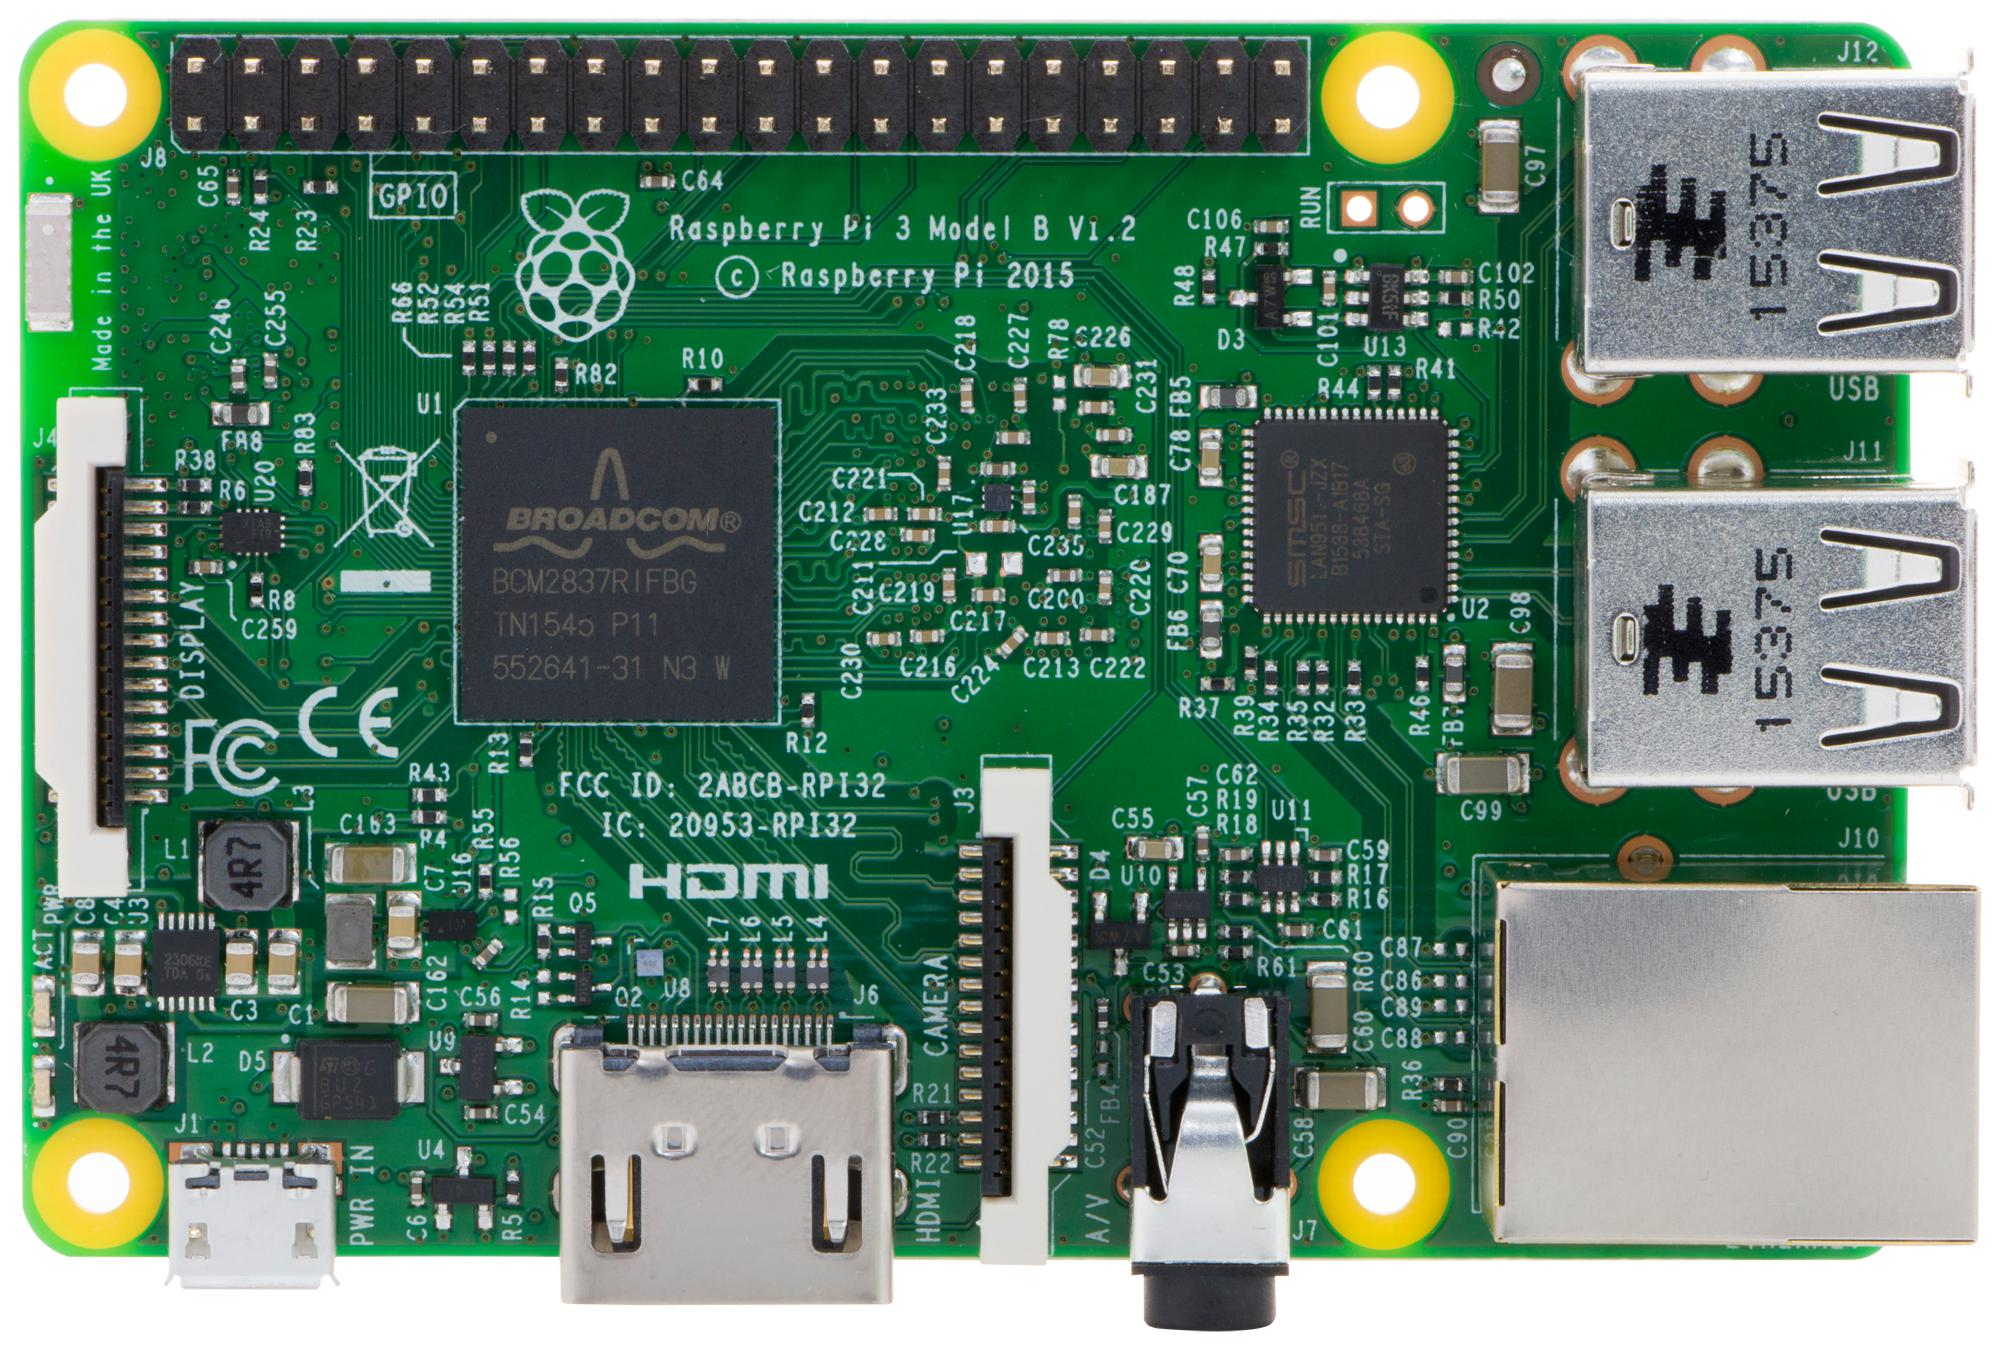
\includegraphics[width=0.4\textwidth]{hardware_pictures/RaspBerryPi 3.jpg}
            \caption{Raspberry Pi 3}
            \label{fig:RaspberryPi}
        \end{figure}
    \item \textbf{Micro Controller}: 32-bit ARM Cortex®-M7 with FPU (216 MHz, 462 DMIPS)
    \item \textbf{Battery}: Lithium polymer 11.1V 1800mAh/19.98Wh 5C (expected operation time: 2u 30min)
    \item \textbf{Actuators}: 2 x Dynamixel XL430-W250
        \begin{figure}[h]
            \centering
            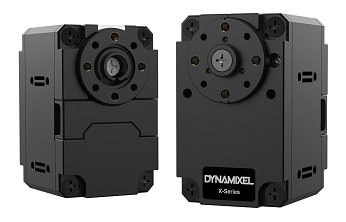
\includegraphics[width=0.5\textwidth]{hardware_pictures/Dynamixel XL430-W250.png}
            \caption{Dynamixel XL430-W250}
            \label{fig:actuators}
        \end{figure}
        
    \newpage
    \item \textbf{Sensor Suite}: Includes a camera and LiDAR for perception and environment monitoring.
    \begin{itemize}
        \item Camera: JetBotRaspberryPiCamera
        \\ The JetBotRaspberryPiCamera is a 12MP camera with a Sony IMX708 sensor. The configured video output is 720p.
            \begin{figure}[h]
                \centering
                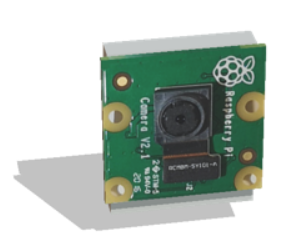
\includegraphics[width=0.3\textwidth]{hardware_pictures/JetBotRaspberryPiCamera.png}
                \caption{JetBotRaspberryPiCamera}
                \label{fig:camera}
            \end{figure}
        \item LiDAR: Robotis LDS-01 
        \\The Robotis LDS-01 is a 1 layer lidar with a range of up to 3.5 meters and a field of view of up to 360 degrees.
        \begin{figure}[ht]
            \centering
            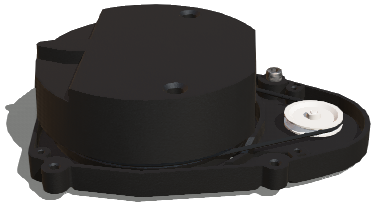
\includegraphics[width=0.4\textwidth]{hardware_pictures/RobotisLds01.png}
            \caption{Robotis LDS-01}
            \label{fig:lidar}
        \end{figure}
    \end{itemize}
\end{itemize}

The complete datasheet of the TurtleBot3 can be found \href{https://www.inf.ed.ac.uk/teaching/courses/sdp/SDP2020/turtlebot3_docs.pdf}{here}

\newpage
\begin{figure}[h]
    \centering
    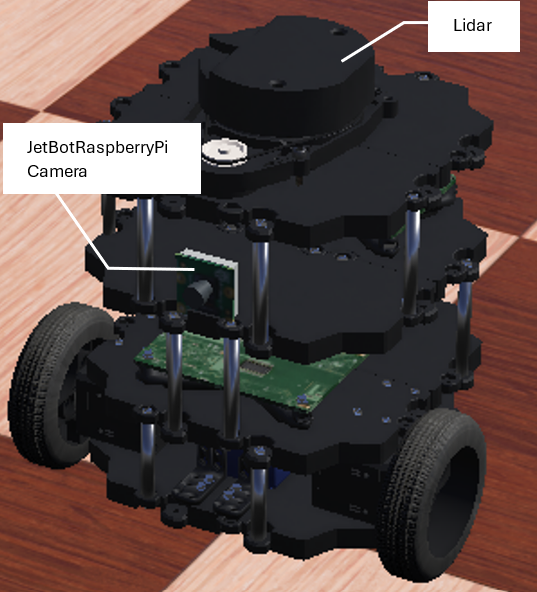
\includegraphics[width=0.7\linewidth]{hardware_pictures/TurtleBot3_hardware.png}
    \caption{TurtleBot3 used for this project}
    \label{fig:turtlebot}
\end{figure}

\newpage
\section{Software Architecture}
The software architecture of the teleoperated robot consists of the following modules:

\begin{itemize}
    \item \textbf{Perception}: Processes sensor data to detect objects and identify obstacles.
    \item \textbf{Input}: Receives commands from the web-based user interface.
    \item \textbf{Movement}: Controls the robot's motion.
    \item \textbf{Output}: Delivers data to the user interface, including LIDAR and video feeds.
    \item \textbf{Controller}: Manages the coordination between different modules.
    \item \textbf{User Interface}: A web-based platform for teleoperation, offering live video feeds, control buttons, and status indicators.
\end{itemize}

\subsection{Perception Module}
The perception module serves as a central unit for collecting and processing sensor data in the robotic system. This module is responsible for integrating data from multiple sensors, specifically a LiDAR sensor and a camera, to provide information that can be used for robotic navigation, obstacle detection, and teleoperation.
\begin{itemize}
    \item \textbf{Initialization}: \\
    Upon initialization, the module activates the LIDAR sensor and the camera. The LIDAR device is set to operate with a frequency of 10 ms and is configured to collect point cloud data. The LIDAR generates a continuous stream of 3D point data for subsequent processing.

    Similarly, the module initializes the camera with a frequency of 10 ms, allowing it to capture images for visual analysis.
    
    \item \textbf{LiDAR Data Processing}: \\
    The perception module provides a method for retrieving the complete point cloud data from the LiDAR sensor. This method returns a list of points, each represented as a set of coordinates (x, y, z). This data can be used to map the surrounding environment, detect obstacles, and aid in navigation.
    
    Additionally, the module includes a method for filtering points based on a specified range. Given a distance in meters, the method identifies and returns only those points that fall within the specified range. This functionality is useful for identifying nearby objects or obstacles and can support obstacle avoidance.
    
    \item \textbf{Camera Data Processing}: \\
    The module incorporates a method for retrieving images from the camera. This method returns the current image captured by the camera, enabling visual feedback. This image data can be used for a variety of purposes, including teleoperation, object recognition, and remote monitoring.
\end{itemize}

\subsection{Input Module}
The input module serves as the interface between the teleoperation interface accessed through a web browser and the robot's control system. Its primary function is to convert user input from the web browser into a standard format compatible with the robot's controller. This approach reduces coupling between the teleoperation interface and the robot's internal components, facilitating modularity and scalability.

\begin{itemize}
    \item \textbf{Validation}: 
    The module verifies that the input data conforms to expected formats and ranges. This step is crucial to ensure that invalid or corrupted data does not affect the robot's behavior. If the input data is invalid or outdated, it is discarded.
    
    \item \textbf{Normalization}: 
    The module standardizes the data to a common format that suits the robot's control system. This process may involve converting units, scaling values, or applying calibration factors to ensure consistent behavior regardless of the source of the input or operating conditions.
\end{itemize}

To ensure non-blocking execution and responsiveness, the module utilizes threading and asynchronous programming. The WebSocket server is launched within a separate thread to prevent blocking the main program execution. Asynchronous functions are used to handle incoming messages, allowing the server to continue listening for new connections and messages while processing existing ones.

Once the input data is processed and validated, the input module generates output commands in a standardized format compatible with the robot's control system. These commands are transmitted to the controller via the communication system, enabling real-time control and supervision of the robot's actions. By decoupling the teleoperation interface from the underlying control logic, the input module promotes modular design principles and facilitates future enhancements or modifications to the system architecture.

\subsection{Movement Module}
The movement module is responsible for controlling the motion of a robot by managing its motor devices and setting speed parameters. It offers methods to move the robot in different directions, considering input signals for forward and lateral movement, as well as an adjustable speed control.
\begin{itemize}
    \item \textbf{Move direction}: \\
     The appropriate velocity for each motor is calculated based on the desired forward and rightward direction vectors. It accounts for both forward and rotational movements, adjusting motor velocities accordingly. The direction vectors are normalized to values between -1 and 1, representing the intensity of movement in the respective directions.
     
    \item \textbf{Speed control}: \\
    This module can set the maximum speed at which the robot can move. By adjusting this parameter, users can control the overall speed of the robot's movements.
\end{itemize}

\subsection{Output Module}
The output module is responsible for streaming sensor data from a robotic system to external clients. It provides a mechanism to share video and LiDAR data over WebSocket connections, allowing real-time monitoring and visualization of the robot's environment. The module integrates separate components for video and LiDAR data streaming, facilitating asynchronous operation and multi-threaded communication.

The output module initializes two separate servers for streaming data:
\begin{itemize}
    \item The video stream server handles video data, converting it to a JPEG suitable for transmitting over WebSocket.
    \item The LiDAR stream server manages LiDAR data, transforming it into JSON format for efficient transmission.
\end{itemize}

Both the video and LiDAR stream servers implement asynchronous data streaming over WebSocket connections. The servers listen for connections from clients and send the stored data when available. This asynchronous approach ensures smooth data transmission without blocking other operations.

\subsection{Controller}
The robot controller oversees the various modules of the robotic system to achieve the desired behaviors. It integrates input, movement, perception, and output functionalities, enabling the robot to interact with its environment and respond to user commands.

The controller runs a main loop, executing a series of actions at each time step to control the robot's behavior.

\begin{itemize}
    \item \textbf{Sensor Data Acquisition}: The controller retrieves LIDAR data to detect nearby obstacles. It also fetches the current camera image for streaming to the user interface.
    \item \textbf{Movement Control}: Based on the input data and sensor readings, the controller directs the robot's movement. If no obstacles are detected within a specific range (0.3 meters), the robot moves according to the input data. If obstacles are detected, the robot stops. Some conditions allow movement if the obstacle's direction does not conflict with the desired input direction.
    \item \textbf{Emergency Stop Handling}: The controller checks for an emergency stop signal from the input module. If activated, the robot's movement is halted to ensure safety.
\end{itemize}

The controller also sends sensor data to the user interface through the output module:
\begin{itemize}
    \item \textbf{Camera Data}: The current camera image is set in the output module, allowing the user to receive live video feeds.
    \item \textbf{LIDAR Data}: LIDAR points within a specified range (3 meters) are streamed to the user interface, providing information on the robot's surroundings.
\end{itemize}

\subsection{User Interface}
    \subsubsection{Video Streaming}
    The BUI incorporates a video streaming component to provide operators with live video feeds from the onboard camera mounted on the robot. This feature enables operators to visually assess the robot's surroundings, identify obstacles, and navigate effectively in real-time.
    
    \begin{itemize}
        \item \textbf{Video Stream Url:}
        Upon loading the BUI, the user inputs the Video stream URL into the designated field and confirms by clicking the ”OK” button
        \item \textbf{WebSocket Integration:}
        To enable seamless video streaming from the robot to the BUI, we employ WebSockets, a powerful communication protocol that facilitates real-time data transmission between clients and servers. By leveraging WebSockets, we establish a persistent connection between the robot and the BUI, allowing for low-latency, high-performance video streaming with minimal overhead.
    
        \item \textbf{Frame Rate Control:}
        To optimize bandwidth usage and ensure consistent video streaming performance, the video streaming component incorporates frame rate control mechanisms. By defining a target frame rate, typically set to 30 frames per second (fps) for smooth playback, the server regulates the rate at which video frames are transmitted to clients.
        Within the WebSocket message handler, a frame rate limiter algorithm monitors the transmission frequency and enforces a minimum inter-frame interval based on the specified frame rate. This ensures that clients receive video frames at a consistent rate, preventing congestion and buffering issues.
        Overall, the video streaming component, implemented using WebSockets, facilitates real-time video transmission from the robot to the BUI, enhancing operators' situational awareness and enabling effective teleoperation in industrial environments.
    \end{itemize}
    
    \subsubsection{Keyboard Input}
    To facilitate teleoperation, the BUI includes keyboard input functionality, allowing operators to control the robot's motion using predefined keyboard commands. By pressing designated keys, operators can maneuver the robot forward, backward, left, and right, providing precise control over its movements.
    \begin{itemize}
    \item \textbf{Vector Generation from Key Input:}
        \begin{itemize}
            \item User key presses are translated into direction vectors for robot movement.
            \item The \texttt{publishKey} function creates a normalized direction vector based on pressed keys.
        \end{itemize}
        
    \item \textbf{Toggling Key Visuals in HTML:}
        \begin{itemize}
            \item Arrow key buttons in the BUI visually toggle to reflect user input.
            \item The \texttt{toggleButton} function dynamically activates or deactivates button visuals.
        \end{itemize}
    \end{itemize}
    
    \subsubsection{Emergency Button}
    The emergency button serves as a critical safety feature, allowing operators to immediately halt the robot's operations in case of emergencies or unexpected situations. The functionality of the emergency button is as follows:
    \begin{itemize}
        \item \textbf{Toggle Emergency State:}
            \begin{itemize}
                \item Clicking the emergency button toggles its state between activated and deactivated.
                \item When activated, the button turns red to visually indicate that the emergency mode is active.
            \end{itemize}
        
        \item \textbf{Sending Emergency Signal:}
            \begin{itemize}
                \item Upon activation, a JSON message containing the emergency status is sent to the robot.
                \item The \texttt{sendData} function is called to transmit the emergency signal to the appropriate topic (\texttt{Robot/emergency}).
            \end{itemize}
    \end{itemize}

\subsubsection{LiDAR Data Visualization}
    The LiDAR data visualization feature enhances the operator's situational awareness by providing real-time information about the robot's surroundings. Here's how it works:

    \begin{itemize}
        \item \textbf{LiDAR Stream Setup:}
            \begin{itemize}
                \item Upon loading the BUI, the user inputs the LiDAR stream URL into the designated field and confirms by clicking the "OK" button.
                \item The \texttt{setupRadarStream} function establishes a WebSocket connection with the LiDAR stream server, enabling data reception.
            \end{itemize}
        
        \item \textbf{Radar Visualization:}
            \begin{itemize}
                \item A radar plot is dynamically generated in the BUI to visualize the LiDAR data.
                \item Each received data point is represented as a dot on the radar plot, indicating the presence of obstacles.
                \item The number of displayed points is limited to 100 for optimization purposes, ensuring smooth performance.
            \end{itemize}
        
        \item \textbf{Color Coding for Distance:}
            \begin{itemize}
                \item Data points closer than 30 centimeters are highlighted in red on the radar plot, signaling potential collision hazards.
                \item This color coding scheme enhances the operator's awareness of nearby obstacles, aiding in navigation and collision avoidance.
            \end{itemize}
    \end{itemize}
\newpage

\subsection{Systems Theoretic Process Analysis (STPA)}

\begin{itemize}[leftmargin=*]
    \item \textbf{Losses and hazards:}
    \begin{itemize}[label=--]
        \item \textbf{Collisions:} The robot collides with an object or a person.
        \item \textbf{Unreliable emergency stop:} The emergency stop functionality fails to operate as intended, causing the robot to not stop in emergency situations.
        \item \textbf{Communication failure:} Unreliable communication between the web application and the robot leads to delays or failures in control signals.
    \end{itemize}
    
    \item \textbf{How/when does the system take actions:}
    \begin{itemize}[label=--]
        \item \textbf{Input:} Commands from the user via the web application.
        \item \textbf{Processes:} Processing of commands by the robot controller, obstacle detection by the LiDAR sensor, and activation of the emergency stop.
        \item \textbf{Output:} Robot movement and feedback to the user via the web application.
        \begin{figure}[h]
            \centering
            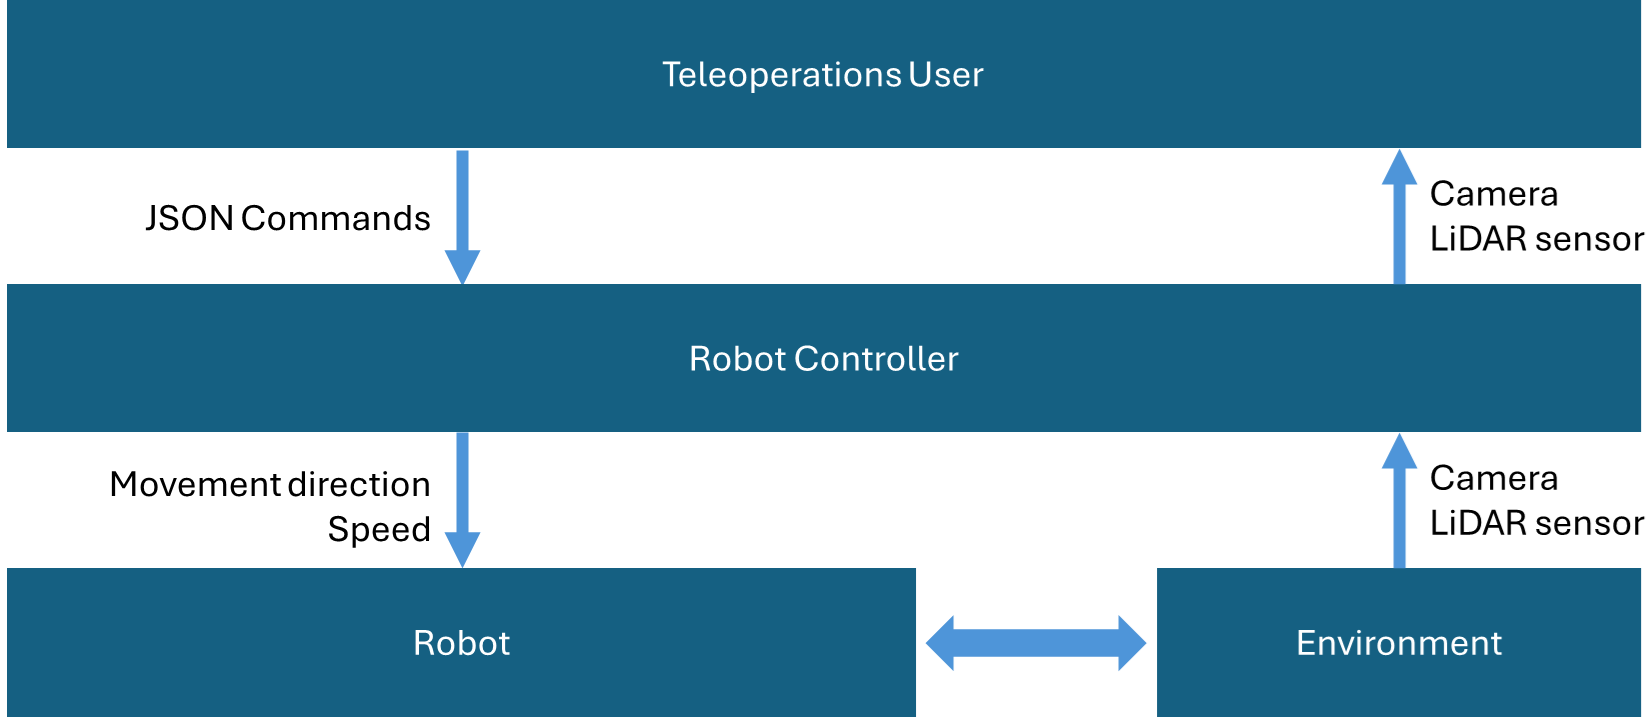
\includegraphics[width=1\linewidth]{Functional_Control_Structure.png}
            \caption{Functional control structure}
            \label{fig:enter-label}
        \end{figure}
    \end{itemize}
    
    \item \textbf{When do these actions lead to bad outcomes:}
    \begin{itemize}[label=--]
        \item Collisions can occur when the robot fails to detect obstacles.
        \item Unreliable emergency stop functionality can lead to delays in emergency situations, increasing the likelihood of a collision.
        \item Communication failures between the web application and the robot can result in delays or errors in control signals, causing the robot to not respond promptly to user commands.
    \end{itemize}
    
    \item \textbf{Why would these actions ever be taken in these circumstances:}
    \begin{itemize}[label=--]
        \item Collisions may occur due to hardware failures, errors in control algorithms, or inadequate obstacle detection by the LiDAR sensor.
        \item Unreliable emergency stop functionality may result from software bugs, hardware errors, or inadequate design of the emergency stop mechanisms.
        \item Communication failures may occur due to network issues, interference, or insufficient security of communication channels.
    \end{itemize}
\end{itemize}

\section{Self-Reflection}
Reflecting on this project, we are pleased with how smoothly everything went. We found the experience with Webots to be quite positive. Its user-friendly interface made it easy to learn, and its wide range of functionalities provided us with the tools we needed to accomplish our goals efficiently.

\subsection{Future Improvements}
Reflecting back on the process, several areas for improvement emerge. Enhancing the robot's autonomy through more sensors coupled with machine learning could reduce the dependency on teleoperation. Additionally, expanding the sensor suite to include additional safety mechanisms, such as ultrasonic sensors or thermal cameras, could further improve safety. Conducting comprehensive tests, including edge cases and stress tests, also could enhance reliability and safety.

\end{document}
